
%(BEGIN_QUESTION)
% Copyright 2007, Tony R. Kuphaldt, released under the Creative Commons Attribution License (v 1.0)
% This means you may do almost anything with this work of mine, so long as you give me proper credit

Calculate the differential pressure sensed by the level transmitter at three different water levels in this boiler steam-drum level measurement system: 0\%, 50\%, and 100\%.

$$\includegraphics[width=15.5cm]{i03612x01.eps}$$

Assume a density for (hot) boiler drum water of 49 lb/ft$^{3}$, a density for steam in the drum of 1.3 lb/ft$^{3}$, and a density for (warm) water in the ``wet leg'' of 61 lb/ft$^{3}$.  If the pressure at the ``low'' (L) side of the transmitter is greater than the pressure at the ``high'' (H) side, be sure to express the differential pressure quantity as a negative number.

\vskip 10pt

\begin{itemize}
\item{} Transmitter $\Delta$P at 0\% water level = \underbar{\hskip 50pt} "W.C.
\vskip 5pt
\item{} Transmitter $\Delta$P at 50\% water level = \underbar{\hskip 50pt} "W.C.
\vskip 5pt
\item{} Transmitter $\Delta$P at 100\% water level = \underbar{\hskip 50pt} "W.C.
\end{itemize}

\vfil 

\underbar{file i03612}
\eject
%(END_QUESTION)





%(BEGIN_ANSWER)

This is a graded question -- no answers or hints given!

%(END_ANSWER)





%(BEGIN_NOTES)

A good way to approach this problem is to treat it the same as a liquid-liquid interface level measurement problem, since the steam's density is great enough to warrant consideration as a pressure-generating fluid in its own right.  Normally, gases and vapors are so sparse that the hydrostatic pressure created by their own weight is negligible.  In this case, however, a weight density of 1.3 lb/ft$^{3}$ is significant enough to warrant inclusion in our hydrostatic pressure calculations.

\vskip 10pt

The wet leg on the transmitter's ``L'' port sees a constant height of 56 inches, filled with water having a density of 61 lb/ft$^{3}$.  This results in a constant ``L'' side pressure (neglecting the static pressure of the steam inside the boiler drum, because we know this static pressure will also be present at the ``H'' port and will therefore cancel as a differential pressure) of 54.74 "WC.

\vskip 10pt

The ``H'' side hydrostatic pressure will be a combination of pressure from the water's height inside the drum (at a reduced density of only 49 lb/ft$^{3}$) plus the pressure resulting from the steam's height inside the drum.  Normally we might treat steam as being a virtually weightless vapor, but in this case its density of 1.3 lb/ft$^{3}$ is significant and so we must factor it into our calculations.

\vskip 20pt

LRV condition = (6 in)(49 lb/ft$^{3}$ / 62.4 lb/ft$^{3}$) + (50 in)(1.3 lb/ft$^{3}$ / 62.4 lb/ft$^{3}$) $-$ (56 in)(61 lb/ft$^{3}$ / 62.4 lb/ft$^{3}$) = {\bf $-$48.99 "WC differential pressure}

\vskip 20pt

URV condition = (46 in)(49 lb/ft$^{3}$ / 62.4 lb/ft$^{3}$) + (10 in)(1.3 lb/ft$^{3}$ / 62.4 lb/ft$^{3}$) $-$ (56 in)(61 lb/ft$^{3}$ / 62.4 lb/ft$^{3}$) = {\bf $-$18.41 "WC differential pressure}

\vskip 20pt

The differential pressure at the 50\% liquid level value will be mid-way between the LRV and URV values: {\bf $-$33.7 "WC differential pressure}


%INDEX% Measurement, level: hydrostatic pressure

%(END_NOTES)


